\section{White box identification}
\subsection{Detached system: cart and springs identification}
To accurately identify the mass of the cart and the stiffness/damping of the spring ,the motor was detached from the cart, in order to reduce influence of friction due to the pinion and rack. \\ \\
So we obtain a system like the one considered in figure \ref{fig:cart_detached_motor}.

\begin{figure}[!h]
\centering
\begin{tikzpicture}[every node/.style={draw,outer sep=0pt,thick}]
\tikzstyle{spring}=[thick,decorate,decoration={zigzag,pre length=0.3cm,post length=0.3cm,segment length=6}]
\tikzstyle{damper}=[thick,decoration={markings,  
  mark connection node=dmp,
  mark=at position 0.5 with 
  {
    \node (dmp) [thick,inner sep=0pt,transform shape,rotate=-90,minimum width=15pt,minimum height=3pt,draw=none] {};
    \draw [thick] ($(dmp.north east)+(2pt,0)$) -- (dmp.south east) -- (dmp.south west) -- ($(dmp.north west)+(2pt,0)$);
    \draw [thick] ($(dmp.north)+(0,-5pt)$) -- ($(dmp.north)+(0,5pt)$);
  }
}, decorate]
\tikzstyle{ground}=[fill,pattern=north east lines,draw=none,minimum width=0.75cm,minimum height=0.3cm]

 
\begin{scope}[xshift=7cm]
\node (M) [minimum width=1cm, minimum height=2.5cm] {$M$};

\node (ground) [ground,anchor=north,yshift=-0.25cm,minimum width=1.5cm] at (M.south) {};
\draw (ground.north east) -- (ground.north west);
\draw [thick] (M.south west) ++ (0.2cm,-0.125cm) circle (0.125cm)  (M.south east) ++ (-0.2cm,-0.125cm) circle (0.125cm);

\node (wall) [ground, rotate=-90, minimum width=3cm,yshift=-3cm] {};
\draw (wall.north east) -- (wall.north west);

\draw [spring] (wall.170) -- ($(M.north west)!(wall.170)!(M.south west)$) node [draw=none,midway,above=0.3cm] {$k$};
\draw [damper] (wall.10) -- ($(M.north west)!(wall.10)!(M.south west)$) node [draw=none,midway,above=0.3cm] {$c$};

\draw [-latex,ultra thick] (M.east) ++ (0.2cm,0) -- +(1cm,0) node [draw=none, midway,above=0.3cm] {$x$};
\end{scope}
\end{tikzpicture}
\caption{Cart detached from the motor diagram.}
\label{fig:cart_detached_motor}
\end{figure}

The differential equation governing this system is given by:
$$M\ddot{x}+c_i\dot{x}+k_i x = f(t)$$
where $M$ [\SI{}{\kilo \gram}] is the total mass of the system  , $c_i$ [\SI{}{\newton \second \per \meter }] comprehends the damping of the $i$-eth spring and the viscous damping of the sliding guide. Finally $k_i$ [\SI{}{\newton \per \meter}] is the stiffness of the $i$-eth spring, and $f(t)$ represents external forces acting on the system (such as non-linear friction components). 
\\ \\
\subsubsection{Experiment description}
For each spring we conducted 2 experiments, one without any load and one with a load of $0.986$ [\si{\kg}], each repeated 3 times. To accurately identify the mass of the cart and the stiffness/damping of the spring ,the motor was detached from the cart, in order to reduce influence of friction due to the pinion and rack. \\\\
For each experiment the  cart was released from an initial condition $x(0) =x_0 \neq 0$ and $0$ velocity,  such that the force that the spring was exerting on the cart was sufficient enough to  make negligible the very small component of the static friction acting on the cart. \\ Notice that the initial condition differs for each spring since the stiffness is very different for each spring. \\\\
If we neglect the external forces acting on the cart, which are negligible since they are small non-linear components, then the system considered is:
\begin{equation} \label{eq:cart_detached_motor}
\begin{cases}
M\ddot{x}+c_i\dot{x}+k_i x = 0 \\
x(0) \in [1,3] \SI{}{\cm} \\
\dot{x}(0)=0
\end{cases}
\end{equation} \\ \\
Then data regarding the position of the cart is collected, and from that data the pulsation, damping ratio, mass and stiffness are retrieved.


\subsubsection{Experiment analysis}
Using \ref{eq:cart_detached_motor} the response in time can be obtained by using the Laplace transform. Let $X(s)$ be the Laplace transform of $x(t)$, then:
$$mX(s)(s^2-x(0)s) +c X(s) (s-x(0)) +kX(s)=0$$
and:
$$X(s) = x(0) \frac{(ms+c)}{ms^2+cs+k}$$
If we solve in $X(s)$ and then apply the inverse Laplace transform, we obtain the response in time:
$$x(t) = e^{-\xi \omega_0 t}(A\cos(\omega t)+B\sin(\omega t))$$
where $\xi = \frac{c}{2\sqrt{Mk}}, \omega_0 = \sqrt{\frac{k}{M}}, \omega = \omega_0 \sqrt{1-\xi^2}$, and $A,B$ depend on $x(0), \xi$. \\ \\
Since the pulsation is the same for both sinusoidal components we have:
$$x(t) = C e^{-\xi \omega_0 t} \sin(\omega t+ \phi)$$
Where  $C= \sqrt{A^2+B^2}, \phi = \arctan(A/B)$.
\\ \\
Knowing those equations we  are able to extract data from the response in the following way:
\begin{itemize}

\item {To measure $\omega$ we can just extract the period $T$:  the difference in time between the first and second peak is taken, and that difference is the period. Then $\omega$ is just $\frac{2\pi}{T}$. We consider only the first and second peak because  at the beginning non-linearities such as static friction are negligible. }

\item {To measure $\xi$ also the first and second peak are considered. Let $t_0, t_1$ be the times at which there is the first and second peak. Notice that $t_0=0, t_1=T$, and $x(T)= Ae^{-\xi \omega_0 T}$.\\
Then, consider:
$$\log \Big(\frac{x(0)}{x(T)}\Big) =  \log(e^{\xi \omega_0 T}) = \xi \omega_0 T = \frac{\xi}{\sqrt{1-\xi^2}} 2\pi$$
Then $$\xi = \frac{a}{\sqrt{a^2+1}}, \quad a = \frac{1}{2\pi}\log \Big(\frac{x(0)}{x(T)}\Big)$$
Once $M,k$ are known we can calculate the damping from $c= 2\xi \sqrt{Mk}$. Observe that for $a \sim 0 \Rightarrow \xi \sim a$. \\ Since damping
}

\item {To identify each spring and the mass of the cart we made use of the fact that the we have two type of experiments for each spring: one without any load, and one with a load of  $0.986$ \SI{}{\kilo\gram}. We obtain a system of linear equations:
$$
\begin{cases}
\frac{k_i}{m_c+m_l} = \omega_l^2 \\
\frac{k_i}{m_c} = \omega_{nl}^2 \\
\end{cases}
$$
Where $m_c$ is the mass of the cart, $m_l$ the mass of the load, $\omega_l$ the pulsation of the system with the load, $\omega_{nl}$ the pulsation of the system without the load. It's a system with two unknowns ($k_i, m_c$) and two equations, so we can solve it. We can rewrite it in matrix form:
$$\begin{bmatrix}
1  && - \omega_l^2 \\
1 && -\omega_{nl}^2
\end{bmatrix}  
\begin{bmatrix}
k_i \\ m_c
\end{bmatrix}  
=\begin{bmatrix}
w_l^2 m_l \\
0
\end{bmatrix}  
$$
and solve for ($k_i, m_c$).
}


\end{itemize}
\subsubsection{Experiment results}
Since there are $3$ springs let's denote the set of springs as $K=\{k_l, k_m, k_h\}$ where \emph{l} stands for low, \emph{m} for medium and \emph{h} for high. In a similar manner we define the various pulsation: for example $\omega_{m-nl}$ is the pulsation for the system with spring $k_m$ and no load.
\\ \\ 
\paragraph{Pulsation}
In the table below are shown the various mean of the pulsation and their relative variance:
\begin{table}[!h]
\centering

\label{table: cart_detached_omega}
\begin{tabular}{|l|l|l|l|}
\hline
{(\textbf{$\omega_{avg}$} [\SI{}{\radian \per \second}],$\omega_{std}$ [\SI{}{\radian \per \second}])} & \textbf{$k_h$} & \textbf{$k_m$}   & \textbf{$k_l$}   \\ \hline
\textbf{with load}         & (21.2989,0 )    & (14.2800 ,    0.0671) & (10.6495 ,0 )      \\ \hline
\textbf{with no load}      & (34.9066 ,0 )    & (23.7101,0.1792) & (17.6991,0.1005) \\ \hline
\end{tabular}
\caption{Pulsation of the cart detached from the motor. Various configuration are shown (with a load of $0.986$ [\SI{}{\kilo \gram}] and no load) for the various springs. }
\end{table} \\ \\
It's interesting to note that even if we considered to average all the periods by considering the various peaks of the signal, and not only the first two peaks, we would have obtained the same results. This is an hint of the fact that the principal non-linearity, i.e. static friction, is negligible.

\begin{figure}[!h]
    \centering
    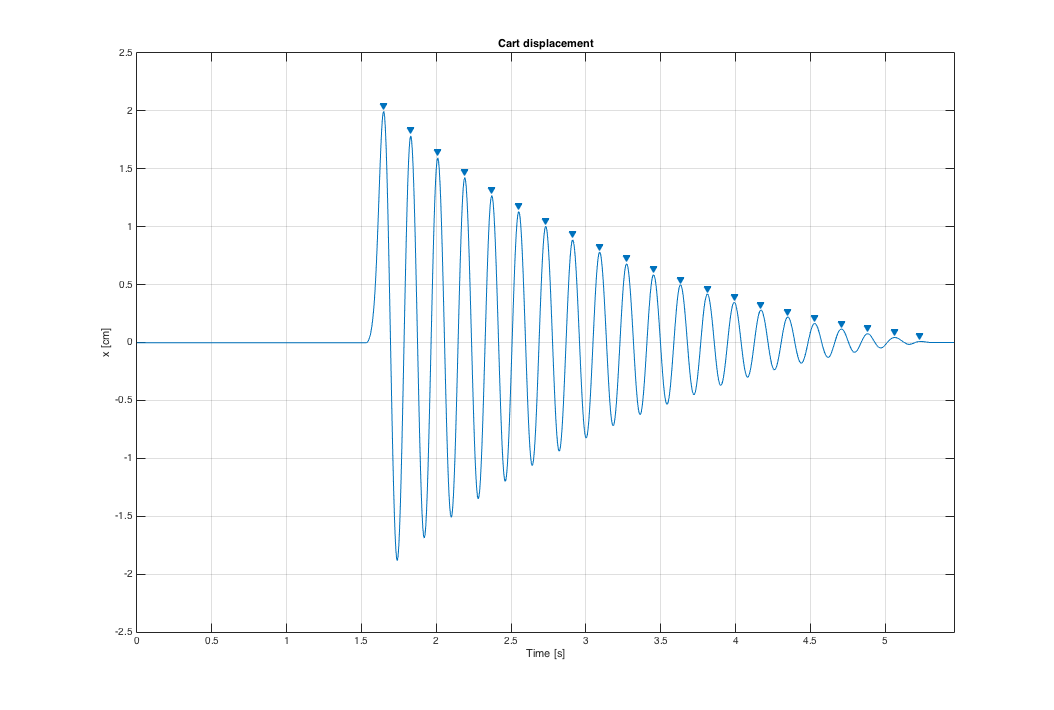
\includegraphics[width=1\textwidth]{img/cart_detached_1.png}
    \caption{Displacement of the cart with spring $k_h$ and load $0.986$ [\SI{}{\kilo \gram}].}
    \label{fig:cart_detached_figure}
\end{figure}
\paragraph{Cart mass and springs stiffness}
By using  the mean pulsation the resultant average mass of the cart $m_c$ is $0.5685$ [\SI{}{\kilo\gram}] with standard deviation $  0.0141$ [\SI{}{\kilo \gram}]. Results also for the springs are shown in table \ref{table: cart_springs_mass}.
\begin{table}[!h]
\centering
\label{table: cart_springs_mass}
\begin{tabular}{|l|l|l|}
\hline
{\textbf{($k_h$ [\SI{}{\newton \per \metre}], $m_c$ [\SI{}{\kilo \gram}])}} & \textbf{($k_m$ [\SI{}{\newton \per \metre}], $m_c$ [\SI{}{\kilo \gram}])} & \textbf{($k_l$ [\SI{}{\newton \per \metre}], $m_c$ [\SI{}{\kilo \gram}])} \\ \hline
(712.5990 ,0.5848)              & (315.5074 ,0.5612 )     & (175.2819,0.5595 )     \\ \hline
\end{tabular}
\caption{Identified springs and cart mass}
\end{table}

\paragraph{Damping and damping ratio}
The mean values for the damping ratio, including their standard deviation, are shown in table \ref{table: cart_detached_dampingratio} for the various springs , with and without the load.
\begin{table}[!h]
\centering

\label{table: cart_detached_dampingratio}
\begin{tabular}{|l|l|l|l|}
\hline
{(\textbf{$\xi_{avg}$},$\xi_{std}$)} & \textbf{$k_h$} & \textbf{$k_m$}   & \textbf{$k_l$}   \\ \hline
\textbf{with load}         & (0.0128,  0.0007 )    & (0.0238, 0.0018) & (0.0346, 0.0036) \\ \hline
\textbf{with no load}      & (0.0179, 0.0025 )    & (0.0301, 0.0013) & (0.0379, 0.0040)      \\ \hline
\end{tabular}
\caption{Damping ratio. Various configuration are shown (with a load of $0.986$ [\SI{}{\kilo \gram}] and no load) for the various springs. }
\end{table}


From the values shown in table \ref{table: cart_detached_damping} it seems that the damping $C$ is function of the mass, in fact we don't obtain the same dampingif we consider the damping ratio with no load or with load. For example consider $k_h$: with a load we obtain $C= 0.0128\cdot2\cdot\sqrt{k_h M}=0.8520$ [\SI{}{\newton \second \per \metre}], without load: $C=0.0179\cdot2\cdot\sqrt{k_h m_c}=0.7206$ [\SI{}{\newton \second \per \metre}]. This is most likely an effect due to friction, and the various damping values are shown in table 
\ref{table: cart_detached_damping}.
\begin{table}[!h]
\centering
\label{table: cart_detached_damping}
\begin{tabular}{|l|l|l|l|}
\hline
{$C$ [\SI{}{\newton \second \per \metre}]} & \textbf{$k_h$} & \textbf{$k_m$}   & \textbf{$k_l$}   \\ \hline
\textbf{with load}         &0.8520    & 1.0542 & 1.1423 \\ \hline
\textbf{with no load}     &0.7206    & 0.8063 & 0.7567      \\ \hline
\end{tabular}
\caption{Damping values. Various configuration are shown (with a load of $0.986$ [\SI{}{\kilo \gram}] and no load) for the various springs. }
\end{table}

We can therefore linearly characterize the damping value as function of the mass centered in $m_c$, for each spring:
$$C(m)=C_{nl}+ \frac{C_{l}-C_{nl}}{m_{l}}(m -m_{c}) = C_{nl} +\alpha (m-m_{c})$$
The different values of $\alpha$, the difference quotient, are shown in table \ref{table: cart_detached_damping_quotient}

\begin{table}[!h]
\centering
\label{table: cart_detached_damping_quotient}
\begin{tabular}{|l|l|l|l|}
\hline
 & \textbf{$k_h$} & \textbf{$k_m$}   & \textbf{$k_l$}   \\ \hline
$\frac{C_{l}-C_{nl}}{m_{l}}$ [\SI{}{\newton \second \per \metre \per \kilo\gram}]       &0.1334   & 0.2514 & 0.3911 \\ \hline
\end{tabular}
\caption{Damping difference quotient. Due to friction damping changes for different weights, we can therefore characterize the damping in a linear way with the formula: $C(m)=C_{nl}+ \frac{C_{l}-C_{nl}}{m_{l}}(m -m_{c})= C_{nl} +\alpha (m-m_{c})$. Values of the difference quotient are shown for the different springs.}
\end{table}



\subsection{Motor identification}

\subsection{Overall system identification}